\cotefile{134-1}
\scanpage{2}

Lettres Breen 75, 76\unsure{.}

% archive sheet number: 1

\scanpage{4}

\noindent\hfill Lodève le 27.\unsure{8.74|8/74|8/4}\\
Cher Deligne,\\
% margin note written sideways
\margin{Cher Breen, J'imagine que tu sais ce que le \unsure{maître|maitre} demande, mais n'ai pu \unsure{neamoins|neanmoins} lui repondre --\\
Qu'en pens-tu. Bien à toi\\
P. \unsure{Deligne}\\}
Étant peut-être empêché \unsure{par ma|par une|par mon} \unsure{faute} d'\unsure{assurer} un cours de 1\textsuperscript{er} cycle au 1\textsuperscript{er} trimestre, je vais peut\unsure{-|'-}être à la place faire un petit séminaire d'algèbre, et envisage de le faire sur les fourbis de Mme Sinh, éventuellement transposés dans le contexte des ``champs''. À ce \unsure{propos}, je tombe sur le truc suivant, qui pour l'instant reste heuristique. Si $M,N$ sont \unsure{deux} faisceaux abéliens sur un topos $X$, et $\tau_{\leq 2}\mathbb{R}\underline{\mathrm{Hom}}(M,N)=E(M,N)$ est le complexe ayant les invariants
\[
\left\{\begin{aligned}
\underline{H}^{i} &= \deleted{\unsure{\mathrm{Hom}}}\underline{\mathrm{Ext}}^{i}(M,N) && \text{pour}\,\unsure{.}\quad 0\leq i\leq 2\\
\underline{H}^{\unsure{j|i}} &= 0 && \text{si}\quad i\notin[0,2]
\end{aligned}\right.
\]
il doit y avoir un triangle distingué canonique
\diagram{\begin{tikzcd}[ampersand replacement=\&,column sep=small,row sep=small]
\& \& {\underline{\mathrm{Hom}}(M,{}_{2}N)[-2]}\arrow[dl] \& \\
(T) \& {E(M,N)}\arrow[rr] \& \& {E'(M,N)}\arrow[ul]
\end{tikzcd}}

% archive sheet number: 61

\scanpage{5}
% Two short horizontal strokes above the first line; hand and purpose uncertain.
\margin{\mbox{-- --}}

donc $E'(M\;N)$ est un complexe dont les invariants $\underline{H}^{i}$ sont ceux de $E(M,N)$ en degré $i\unsure{\ne|+}2$, et qui en degré $2$ donne lieu : une suite exacte
\begingroup
\makeatletter\tagsleft@true\makeatother
\[
\tag*{(\unsure{S|*})}
0\to\underline{\mathrm{Ext}}^{2}(M,N)\to
\overbrace{\underline{H}^{2}\!\left(E'(M,N)\right)}^{P(M,N)}
\xrightarrow{\sigma}\underline{\mathrm{Hom}}(M,{}_{2}N)\to \unsure{0}
\]
\endgroup

Heuristiquement, $E'(M,N)$ est le complexe qui exprime le ``2-champ de Picard\deleted{\unsure{''|*}} strict'' formé des 1-\unsure{champs|champ} de Picard (pas \unsure{nécessairement} stricts) \inserted{``épinglés'' par $M,N$} sur des objets variables de $X$, en admettant que ta théorie pour les 1-champs de Picard \inserted{stricts} s'étend aux 2-champs de Picard stricts (ce qui pour \unsure{,|.} moi ne fait guère de doute) ; de même $E(M,N)$ correspond aux champs de Picard \uline{stricts} épinglés par $M,N$.

La suite exacte $(*)$ se construit en \unsure{tous|tout} cas canoniquement ``à la main'', où \unsure{\deleted{le}|le} terme médian est le faisceau des \unsure{classes|données} \inserted{à} \deleted{\unsure{d'|à}}``équivalence'' près des

% Two curved, nonlexical impressions and adjacent edge dots at the lower left of the copied sheet.
% The small possible comma before moi is retained uncertainly; it may be a copying fleck.
% archive sheet number: 62

\scanpage{6}
% Two short horizontal strokes at the upper right.
\margin{\mbox{-- --}}

\deleted{\unsure{catégories|catégorie}}\inserted{champs} de Picard \unsure{épinglés|épinglées} par $M.N$, $\sigma$ étant l'invariant qui \inserted{s'obtient en\unsure{,}} associant à toute section \inserted{$L$} d'un champ de Picard la symétrie de $\deleted{\unsure{N|L}}L\otimes L$, \unsure{interprétée} comme section de ${}_{2}N$. Je sais prouver (sauf erreur) que tout hom. $M\to{}_{2}N$ provient d'un champ de Picard convenable (épinglé par $M,N$) (a priori l'obstruction est dans $\mathrm{Ext}^{3}(X;M,N)$, mais un argument ``\unsure{universel|universal}'' prouve qu'elle est nulle). Cela prouve que l'extension $(*)$ est bien proche d'être splittée : \deleted{\unsure{la|un}} tte section du troisième faisceau, sur un objet quelconque de $X$, se remonte -- en d'autres termes l'extension a une section ``ensembliste''. Bien sûr, il y a mieux en fait : toute section sur un $U\in\mathrm{Ob}\,X$ ``provient'' d'un élément de $\mathscr{H}^{2}(U,{\unsure{\underline{F}|E}}'(M\unsure{.}N\unsure{;|)|,}))$\unsure{.} (hypercohomologie $\mathscr{H}^{2}$).

% archive sheet number: 63

\scanpage{7}

\uline{\illegible{1}}\unsure{:|,} \unsure{soit} $\unsure{\mathcal{A}|\mathscr{A}|A}$ un anneau sur $X$, soient $M,N$ respectivement les faisceaux $K^{0}$ et $K^{1}$ associés au champ additif des $\mathcal{A}$-Modules projectifs de v. f. \inserted{(\unsure{p|par} ex.)\unsure{!|;|,}} Alors la \unsure{construction} de Mme Sinh nous fourni un champ de Picard \unsure{e|é}pinglé par $M,N$, d'où une section \deleted{\unsure{du|de}} canonique du terme médian $\unsure{P|F}(M,N$ de $(*)$.

\uline{NB} Tout ce qui précède a les \unsure{fonctorialités} évidentes en $M,N,X$\ldots

\uline{Question} : Le triangle exact $(\unsure{J|T})$ \unsure{et} la suite exacte $(\unsure{*})$ sont ils \unsure{connu|connus} par les comp\unsure{è|é}tences (Quillen, Breen Illusie\ldots) ? \unsure{Connaissent-ils|Donnaissent-ils} des \unsure{variantes|variante} ``supérieures'' ? (Un principe ``géométrique'' pour en obtenir pourrait être via des $n$-champs de Picard non néc. stricts\ldots)

% Isolated raised points above the question sequence label and between ils and connu have no established textual function.
% Two curved impressions run along the lower left edge of the copied sheet.
% archive sheet number: 64

\cotefile{134-2}
\scanpage{146}\mspage{1}
\hfill Villecun 17/19 \unsure{Juillet|juillet}\unsure{.}\\
\hfill 1975\\
Cher Larry,\\

Tout d'abord félicitations pour la naissance de ta fille, qui heureusement ne s'est pas laissée impressionner par les importantes cogitations mathématiques de son papa -- au risque de les perturber quelque peu.

Au fait, quelle est ta situation en France : es\deleted{\unsure{t}}-tu français ou américain, prof. associé ou titulaire ? Si cela pouvait s'arranger, \unsure{serait|serais} tu intéressé par une position : Montpellier ? Cela te dit-il quelque chose de venir à l'occasion à Montpellier -- ou à Villecun -- pour discuter de tes \unsure{favoris|fantaisies} avec moi -- pour le moment il n'y a guère que moi ici pour ne pas nager entièrement (seulement partiellement) dans ce que tu fais.

J'ai été content de finir par recevoir un écho à ma longue \unsure{è|é}pitre -- et même un début d'approche constructive pour \deleted{\unsure{une structure}} une théorie du type que je prévois. La construction que tu proposes de la notion de $n$-catégorie pas stricte, et du foncteur nerf, a certes le mérite \inserted{d'exister et} d'être une premièr approche précise, mais par ailleurs prête \deleted{\unsure{naturellement|évidemment}} \inserted{bien sûr}, le flanc à des critiques évidentes : d'être très technique, peu intuitive (alors \unsure{qu'au|où au} niveau des $1$-cat. et
% archive sheet number: 146

\scanpage{147}\mspage{2}
\={m} des $2$-cat. tout parait si clair -- ``il n'y a qu'à suivre le bout de son nez''\dots) et enfin l'absence d'une définition d'un foncteur allant des ens. (semi) simpliciaux vers les $n$-groupoïdes. Ce foncteur correspond à une intuition géométrique si claire qu'une théorie qui ne l'inclurait pas me semblerait canularesque. Peut-être en \inserted{essayant d'}écri\deleted{\unsure{vant}}\unsure{re} (Comme\unsure{:|.} une sorte de liste de voeux de Noël !) de façon assez complète et explicite les \deleted{relations} notions \deleted{\unsure{qu'on}}dont on voudrait disposer et les relations (foncteurs, équivalences etc) qui doivent les lier, arriverait-on finalement à une sorte de description axiomatique assez poussée \deleted{\unsure{pour}}qui, soit \unsure{donne|donner} la clef d'une construction ad-hoc explicite, soit \inserted{qui permette} à la rigueur d'énoncer et démontrer un th. d'existence et d'unicité d'une théorie du type souhaité.

Par ailleurs, n'ayant pas compris l'idée de Segal dans ta dernière lettre (que j'ai généreusement envoyée à Illusie\dots), je ne vois pas comment tu définis les $n$-cat. de Picard -- mais peu importe. Pour ce qui est des $n$-cat. de Picard ``strictes'', tout ce que je leur demande, c'est qu'ils forment finalement une \inserted{$(n+1)$-}catégorie $(n+1)$-équivalente à celle des complexes de chaines de longueur\unsure{,} $n$. D'accord ? Je te remercie
% archive sheet number: 147

\scanpage{148}\mspage{3}
d'avoir rectifié dans mon esprit une erreur grossière, dû à ma grande ignorance de la top. algébrique et de l'homotopie -- j'étais en effet dans le sentiment que les $H$-espaces satisfaisant des conditions d'associativité et commutativité assez strictes (disons équivalent à des $\unsure{{}'}\!\Omega^{i}X$ avec $i$ arbitrairement grand) correspondaient à des\unsure{.} groupes topologiques \unsure{commutatifs|commutatif} (en m'inspirant de quelques analogies \dots). Donc entièrement d'accord avec tes observations p.~5.\unsure{.}

Par contre, je suis toujours intrigué par la question suivante : n'y\unsure{.} a-\unsure{t-il|til} pas un analogue du tapis de Dold-Puppe pour les groupes ($1/2$) simpliciaux (pas néc. commutatifs) et quelle forme prend-il ? À vrai dire, je considère le yoga
\diagram{\begin{tikzcd}[ampersand replacement=\&]
\text{ens. }1/2\text{ simplicial}\arrow[leftrightarrow,r] \& \infty\text{-}\deleted{\unsure{\text{catégorie}}}\text{groupoïde}
\end{tikzcd}}
comme étant essentiellement la version ``set-theoretic'' ultime de Dold-Puppe, qui s'en déduirait en explicitant seulement que les groupes abéliens dans $(\infty\text{-cat})$ ne ``sont autres'' que les complexes de chaines dans $(\mathrm{Ab})$. Il faudrait donc déterminer quels sont les groupes de $(\infty\text{-cat})$ : Je peux te dire ce qu'il en est dans $(1\text{-cat})$ -- ce sera \unsure{dévelop|divulg}%
% The manuscript has a terminal line-end hyphen after the incomplete final word.
% archive sheet number: 148

\scanpage{149}\mspage{4}%
% First occurrence of strictes: one wavy underline; second occurrence: one straight underline.
pé en long et en large dans le livre de Mme Sinh, je pense, sous le titre de chapitre des ``Gr-catégories \uline{strictes}'' (i.e. \inserted{\unsure{où}} les isomorphismes d'associativité, d'unité, et d'inverse $X\mathbin{.}X^{-1}\unsure{\simeq|=}1$ sont des \uline{identités}). On peut expliciter p.ex. comment (via le fait que tte Gr-cat. est Gr-équivalente à une Gr-catégorie stricte) le calcul avec les Gr-catégories se \unsure{réduit} à un calcul très algébrique avec des Gr-catégories \uline{strictes}, par une sorte de ``calcul des fractions'' (à droite ou à gauche, au choix) du type de celui qui aboutit à la construction des catégories dérivées. Quoi qu'il en soit, voici l'explicitation de cette structure (groupe dans $(1\text{-ct.})$) en termes de théorie des groupes ($1$-catégorie dans $(\mathrm{Gr})$) :

La structure est décrite par un \unsure{.} quadruplet $(L_1,L_0,d,\unsure{\Theta|\theta})$, avec
\diagram{\begin{tikzcd}[ampersand replacement=\&]
L_1 \arrow[r,"d"] \& L_0\,\raisebox{1.1ex}{$\scriptstyle\unsure{:}$}
\end{tikzcd}}
un hom de groupes ordinaires, et
\[
\Theta:L_0\longrightarrow\underline{\mathrm{Aut}}_{\mathrm{gr}}(L_1)
\]
une opération de $L_0\deleted{\unsure{\Theta|\theta|0}}$ sur $L_1$, avec les
% archive sheet number: 149

\scanpage{150}\mspage{5}
deux axiomes suivants

a) $d$ commute aux op. de $L_0$, quand on le fait opérer sur $L_1$ par $\unsure{\Theta|\theta}\deleted{\unsure{s|,}}$, sur lui-même par aut. int :
\[
d\bigl(\Theta(x_0)\mathbin{.}x_1\bigr)=\mathrm{int}(x_0)\,d(x_1)
\]
\[
\Theta(d.(x_1))=\mathrm{int}(x_1)\tag*{\makebox[0pt][r]{\makebox[\displaywidth][l]{b)}}}
\]
Ces propriétés impliquent que $\mathrm{Im}\,d$ est \unsure{invariant} dans $L_0$ (donc $\unsure{\mathrm{Coker}|\mathrm{CoKer}}\,d=\unsure{\pi|\Pi}_0$ est défini) et $\pi_1=\mathrm{Ker}\,d$ est central dans $L_1$, enfin que $L_0$ opère sur $L_1$ en invariant $\pi_1$, et qu'il opère via $\pi_0$. Le principal invariant \inserted{coh.} de la situation est évidemment l'inv. de \unsure{Postnikoff|Postnikuff}-Sinh
\[
\alpha\in\unsure{.}\,H^3(\pi_0,\pi_1).
\]

J'ai rencontré ces animaux -- sans même les chercher -- dans pas mal de situations, que je ne vais pas te passer en revue ici (je viens d'ailleurs de \unsure{retomber} encore dessus à propos de la classification des groupes formels ``ordinaires'' \unsure{sur|\deleted{\illegible{1}}sur} un corps parfait, en termes de groupes alg\unsure{è|é}briques \uline{affines}\unsure{,|;} de groupes formels \uline{commutatifs}, reliés par des Gr-structures strictes de ce type%
% margin note written sideways; the guide ends beside the line beginning strictes, without an exact word anchor
% The guide below is reproduced in the original page orientation; the note text is read upright.
\margin{\illegible{4} ce formalisme sur un topos quelconque (pas seulement dans $(\mathrm{Ens})$)
\figure{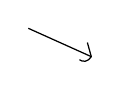
\begin{tikzpicture}[x=1cm,y=1cm]
\draw[line width=.45pt] (0,.36) -- (.80,0);
\draw[line width=.45pt] (.75,.18) -- (.80,0) .. controls (.76,-.07) and (.69,-.07) .. (.65,-.04);
\end{tikzpicture}}} -- pour expliciter le yoga que ``le \unsure{caractêre|caractère} transcendant \unsure{des|du}
% archive sheet number: 150

\scanpage{151}\mspage{6}
\unsure{groupe|groupes} \unsure{formel|formels} est concentré en les groupes formels commutatifs, découvert semble-t-il par Dieudonné \dots). La question que je voudrais soulever est la généralisation aux groupes dans $(n\text{-cat})$, on s'attend à trouver des complexes de chaines non comm
\diagram{\begin{tikzcd}[ampersand replacement=\&,column sep=small]
L_n\arrow[r,no head,to path={-- (\tikztotarget) -- ++(0.025,0.055)}] \& L_{n-\unsure{,|1}}\arrow[r,no head,to path={-- (\tikztotarget) -- ++(0.025,0.055)}] \& \ldots\arrow[r,no head,to path={-- (\tikztotarget) -- ++(0.025,0.055)}] \& L_1\arrow[r,no head,to path={-- (\tikztotarget) -- ++(0.025,0.055)}] \& L_0\arrow[r] \& 1
\end{tikzcd}}
avec des structures supplémentaires sans doute du type $\unsure{\Theta|\theta}$, mais lesquelles ? Il est entendu que la signification topologique de ces structures, c'est qu'elles expriment exactement les ``types d'homotopie tronqués en dim $\leq n$'' des groupes topologiques. \inserted{\unsure{mesurant} les types d'hom \unsure{tronqués|tronques|tr. \deleted{qués}} en dim $\leq n+1$ des espaces top ponctu\unsure{e|é}s connexes \dots)}
% Guide of the preceding interlinear addition: its left end is before As-tu.
\figure{\begin{tikzpicture}[x=1cm,y=1cm]
\draw (0,0) .. controls (-0.08,0.30) and (-0.05,0.48) .. (0.20,0.53) .. controls (0.90,0.64) and (2.90,0.47) .. (3.30,0.60) -- (3.32,0.72);
\node[inner sep=0pt] at (0.27,0.38) {\unsure{.}};
\end{tikzpicture}}
As-tu des \unsure{candïdats|candidats} à proposer ?

\figure{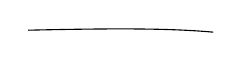
\begin{tikzpicture}\draw (0,0) .. controls (1.1,0.025) and (1.8,0.025) .. (2.35,-0.025);\end{tikzpicture}}

% Guide beneath et d'homologie; the left leg attaches after bidualité.
\figure{\begin{tikzpicture}[x=1cm,y=1cm]
\draw (0,0) -- (0.24,0.64) .. controls (1.20,0.68) and (2.68,0.56) .. (3.45,0.53) -- (3.44,0.65);
\end{tikzpicture}}
\unsure{.} Tes réflexions de bidualité \inserted{et d'homologie}, pour formelles qu'elles soient, se rattachent à une foule de développements, dont certains seulement existent\unsure{,} d\unsure{è|é}s \unsure{â|à} présent, et d'autres demanderaient des développements considérables. Voici les réminiscences que m'ouvrent tes \unsure{noïves|naïves} questions :
% archive sheet number: 151

\scanpage{152}\mspage{7}%
A) Le formalisme des $Rf_!, f^!$ (combiné à $Rf_*, Lf^{\alpha}$, $\overset{\mathbb{L}}{\otimes}$ et $\mathbb{R}\mathrm{Hom}$, ``les six opérations'') porte implicitement en son sein la définition de l'homologie et l'identité essentielle entre \unsure{fonctions} homologiques et cohomologiques. \deleted{\unsure{E}} On dispose pour le moment de ce formalisme pour les faisceaux quasi-cohérents sur les schémas -- séminaire Hartshorne -- pour les espaces top. et les faisceaux de coeff. arbitraires dessus -- Verdier, exposé Bourbaki -- et en coh. étale des schémas pour les coefficients ``discrets'' \inserted{(de torsion ou ``$l$-adiques'')}
% Source guide below the parenthetic addition: long upper arm, short left descent beside premiers, and right upturn; no arrowhead. The separate lower crossed stem belongs to f in faisc.
\figure{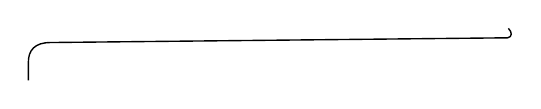
\begin{tikzpicture}[x=0.01cm,y=-0.01cm]
\draw[line width=0.5pt] (610,0) .. controls (615,5) and (615,11) .. (609,12)
 -- (28,18) .. controls (8,18) and (0,28) .. (0,43) -- (0,66);
\end{tikzpicture}}
\uline{premiers a\unsure{\.{u}|u}x \deleted{\unsure{la|le}} car. résiduelles} -- SGA 5 --
% The right guide lies above the added analytic case and descends from after SGA 5 into the space above the names. Its semicolon is reproduced inside the bend, not assigned an invented baseline order.
\figure{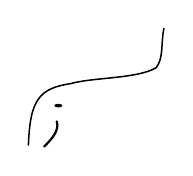
\begin{tikzpicture}[x=0.02cm,y=-0.02cm,line cap=round,line join=round]
\draw[line width=0.55pt] (89,2) .. controls (87,11) and (89,21) .. (84,27) .. controls (72,34) and (44,33) .. (30,37) .. controls (10,40) and (4,47) .. (3,76);
\fill (22,51) ellipse [x radius=2.6,y radius=1.15];
\draw[line width=0.8pt] (21,61) .. controls (23,67) and (17,73) .. (13,77);
\end{tikzpicture}}
\inserted{enfin pour les faisc. coh. sur les espaces analytiques -- Verdier-\unsure{Rüget|Ruget|Rüguet|Ruguet} --}
% The addition is slightly slanted in the source.
(Le formalisme reste à développer dans le contexte cristallin, et en car. $0$ dans le contexte des modules stratifiés \inserted{à singularités}
% Guide immediately below singularités, with an uncertain detached point to its left below early stratifiés. The g descender above is separate from the guide.
\figure{\begin{tikzpicture}[x=0.01cm,y=-0.01cm]
\path[use as bounding box] (0,65) rectangle (577,136);
\node[inner sep=0pt] at (88,113) {\unsure{.}};
\draw[line width=0.5pt] (363,127) .. controls (353,96) and (359,79) .. (401,75)
 .. controls (423,71) and (437,72) .. (448,76)
 .. controls (491,94) and (544,98) .. (567,94);
\end{tikzpicture}}
à la Deligne, avec éventuellement -- sur le corps $\mathbb{C}$ -- des structures de Hodge à la clef, enfin dans le contexte des motifs ; je suis persuadé qu'il est présent
% The small doubtful point stands below the beginning of un, rather than after the word.
\makebox[0pt][l]{\hspace{0.1em}\raisebox{-1.4ex}[0pt][0pt]{\unsure{.}}}un peu partout encore -- partout, peut-\unsure{\={e}tre|être}, où il y a un formalisme de nature cohomologique.) Travaillant en coh. étale sur un schéma \inserted{séparé}
% Guide immediately below séparé: curved left descent before de, rising arm, and small terminal hook at upper right.
\figure{\begin{tikzpicture}[x=0.02cm,y=-0.02cm,line cap=round,line join=round]
\draw[line width=0.55pt] (14,70) .. controls (3,55) and (3,40) .. (19,34) .. controls (40,25) and (82,19) .. (105,9) .. controls (114,5) and (110,0) .. (102,3);
\end{tikzpicture}}
de t.f. sur un corps $k$, disons,
% Detached point beneath the initial portion of avec; intent uncertain.
\makebox[0pt][l]{\hspace{0.1em}\raisebox{-1.4ex}[0pt][0pt]{\unsure{.}}}avec un anneau de \unsure{coeff.|coeff} $\Lambda$ de \unsure{torsion} \unsure{premier} à \unsure{la} \unsure{car}
% The last baseline is cut by the lower edge; no final punctuation is recoverable.
% archive sheet number: 152
